\chapter{Introduction}\label{chap:introduction}
\section{Galaxy workflows}
A Galaxy workflow is a sequence of tools to process biological data. In this sequence, Galaxy tools are connected one after another forming a data processing pipeline. The linked tools in a workflow have compatible datatypes which means that the output datatype of one tool should be consumable by the next tool. A workflow can also be inferred as a directed acyclic graph. Figure 33 shows a workflow containing two paths. In general, a workflow can have multiple paths between its input and output tools. Each of these paths has a direction commencing from an input tool and ending at an output tool. Moreover, the paths in a workflow can have one or more tools in common. We can see in the figure 33 that tools like "Get flanks", "AWK" and "Intersect" are common in both the paths.

\begin{figure}[h]
\begin{centering}
    {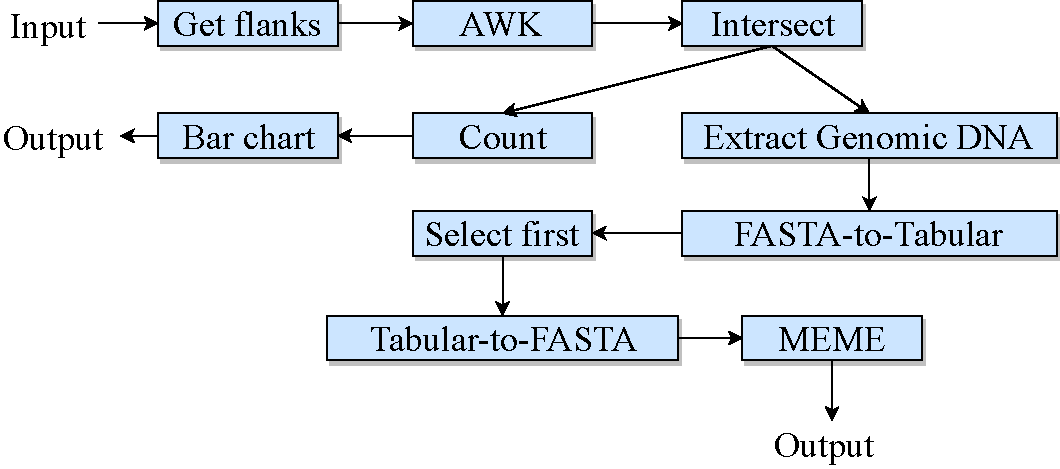
\includegraphics[scale=0.7]{figures/simple_wf_45cee2961bc05b20.pdf}}
    \caption[A workflow]{\textbf{A workflow}: The image shows a workflow with two paths. It takes input data, processes it through multiple steps involving many tools in both the paths, a few tools being common, and gives two outputs.}
\end{centering}
\end{figure}

While creating a workflow, at each stage, a user chooses a tool from clusters of tools and connect it to the previous tool. The user repeats this until a desired stage of output is reached. In each of these stages, a tool can connect to one or more tools which are compatible to the previous tool. A user needs to decide which tool to connect next which depends on the multiple factors like the kind of input data, the nature of processing and so on.